%% This section adds chapter 1
\section{Introduction}
% example entries for nomenclature. These entries should be given throughout the text right after the symbol is used the first time. If "refpage" option is given, the corresponding page number is shown in nomenclature. The following nomenclature groups are used; A=Latin, B=Greek, C=Subscripts, D=Superscripts, E=Abbreviations, F=Dimensionless. This letter code should be placed first inside the [] brackets. The following letters inside square brackets [] are used to alphabetically sort the symbols and abbreviations in the list. The symbol or abbreviation itself is defined within the curly braces {} after the square brackets. The $$ signs create an equation form, i.e. a variable in italics. Inside the latter brackets, the legend and the unit are defined with the \nounit{} definition. For units, italics can be removed with the \mathrm{} command. See instructions https://www.overleaf.com/learn/latex/Nomenclatures or https://www.ctan.org/pkg/nomencl. 
% A=Latin letters
\nomenclature[Aa1]{$A$}{area\nomunit{$\mathrm{m^2}$}}
\nomenclature[Aa2]{$a$}{constant}
\nomenclature[Acd]{$C_D$}{drag coefficient}
\nomenclature[Acp]{$c_p$}{specific heat capacity at constant pressure\nomunit{$\mathrm{J/(kgK)}$}}
\nomenclature[Acv]{$c_v$}{specific heat capacity at constant volume\nomunit{$\mathrm{J/(kgK)}$}}
\nomenclature[Ad]{$d$}{diameter\nomunit{$\mathrm{m}$}}
\nomenclature[AF]{$\mathbf{F}$}{force vector\nomunit{$\mathrm{N}$}}
\nomenclature[Af]{$f$}{frequency\nomunit{$\mathrm{1/s,Hz}$}}
\nomenclature[Ag]{$g$}{acceleration due to gravity\nomunit{$\mathrm{m/s^2}$}}
\nomenclature[Ah]{$h$}{heat transfer coefficient\nomunit{$\mathrm{W/(m^2K)}$}}
%\nomenclature[Ah2]{$h$}{specific enthalpy\nomunit{$\mathrm{J/kg}$}}
\nomenclature[Aj]{$\mathbf{j}$}{flux vector\nomunit{$\mathrm{m/s}$}}
\nomenclature[AL]{$L$}{characteristic length\nomunit{$\mathrm{m}$}}
\nomenclature[Al]{$l$}{length\nomunit{$\mathrm{m}$}}
\nomenclature[AM]{$M$}{torque\nomunit{$\mathrm{Nm}$}}
\nomenclature[Am]{$m$}{mass\nomunit{$\mathrm{kg}$}}
\nomenclature[AN]{$N$}{number of particles}
\nomenclature[An2]{$\mathbf{n}$}{unit normal vector}
\nomenclature[Ap]{$p$}{pressure\nomunit{$\mathrm{Pa}$}}
\nomenclature[Aq]{$q$}{heat flux\nomunit{$\mathrm{W/m^2}$}}
\nomenclature[Aqm]{$q_m$}{mass flow rate\nomunit{$\mathrm{kg/s}$}}
\nomenclature[Ar]{$r$}{radius\nomunit{$\mathrm{m}$}}
\nomenclature[AT]{$T$}{temperature\nomunit{$\mathrm{K}$}}
\nomenclature[At]{$t$}{time\nomunit{$\mathrm{s}$}}
\nomenclature[AV]{$V$}{volume\nomunit{$\mathrm{m^3}$}}
\nomenclature[Av]{$v$}{velocity magnitude\nomunit{$\mathrm{m/s}$}}
\nomenclature[Av2]{$\mathbf{v}$}{velocity vector\nomunit{$\mathrm{m/s}$}}
\nomenclature[Ax]{$x$}{x-coordinate (width)\nomunit{$\mathrm{m}$}}
\nomenclature[Ay]{$y$}{y-coordinate (depth)\nomunit{$\mathrm{m}$}}
\nomenclature[Az]{$z$}{z-coordinate (height)\nomunit{$\mathrm{m}$}}
% B=Greek symbols
%\nomenclature[Ba]{$\alpha$}{thermal expansion coefficient\nomunit{$\mathrm{1/K}$}}
\nomenclature[Ba]{$\alpha$}{(alfa)\nomunit{$\mathrm{1/K}$}}
\nomenclature[Bb]{$\beta$}{(beta)}
\nomenclature[BG]{$\Gamma$}{(Gamma)}
\nomenclature[Bg]{$\gamma$}{(gamma)}
\nomenclature[BD1]{$\Delta$}{(Delta) usually used for change/difference}
\nomenclature[BD2]{$\varDelta$}{(varDelta)}
\nomenclature[Bd3]{$\delta$}{(delta) notice the difference to $\partial$ (partial differential)}
\nomenclature[Be1]{$\epsilon$}{(epsilon)}
\nomenclature[Be2]{$\upepsilon$}{(upepsilon)}
\nomenclature[Bz]{$\zeta$}{(zeta)}
\nomenclature[Be3]{$\eta$}{(eta)}
\nomenclature[Bth]{$\theta$}{(theta)}
\nomenclature[BTh]{$\Theta$}{(Theta)}
\nomenclature[Bth2]{$\vartheta$}{(vartheta)}
\nomenclature[Bi]{$\iota$}{(iota)}
\nomenclature[Bk]{$\kappa$}{(kappa)}
\nomenclature[BL]{$\Lambda$}{(Lambda)}
\nomenclature[Bl]{$\lambda$}{(lambda)}
\nomenclature[Bm]{$\mu$}{(mu)}
\nomenclature[Bm2]{$\upmu$}{(upmu)}
\nomenclature[Bn]{$\nu$}{(nu)}
\nomenclature[BX]{$\Xi$}{(Xi)}
\nomenclature[Bx]{$\xi$}{(xi)}
\nomenclature[BP]{$\Pi$}{(Pi)}
\nomenclature[Bp]{$\pi$}{(pi) e.g. pressure ratio, note the difference with (uppi) constant $\uppi=3.14\ldots$}
\nomenclature[Br]{$\rho$}{(rho)}
\nomenclature[Br2]{$\uprho$}{(uprho)}
\nomenclature[BS]{$\Sigma$}{(Sigma)}
\nomenclature[Bs]{$\sigma$}{(sigma)}
\nomenclature[Bs2]{$\varsigma$}{(varsigma)}
\nomenclature[Bta]{$\tau$}{(tau)}
\nomenclature[Bu]{$\upsilon$}{(upsilon)}
\nomenclature[Bph]{$\phi$}{(phi)}
\nomenclature[BPh]{$\Phi$}{(Phi)}
\nomenclature[Bph2]{$\varphi$}{(varphi)}
\nomenclature[BX]{$\chi$}{(chi)}
\nomenclature[BPs]{$\Psi$}{(Psi)}
\nomenclature[Bps]{$\psi$}{(psi)}
\nomenclature[BO]{$\Omega$}{(Omega)}
\nomenclature[Bo]{$\omega$}{(omega)}
% C=Subscripts
\nomenclature[Ce]{eff}{effective}
\nomenclature[Cma]{max}{maximum}
\nomenclature[Cmi]{min}{minimum}
\nomenclature[Cg]{g}{gas}
\nomenclature[Ct]{tot}{total}
\nomenclature[Cp]{p}{particle}
\nomenclature[Cs]{s}{solid}
\nomenclature[Cl]{l}{liquid}
% D=Superscripts
\nomenclature[Dp]{p}{partial layer}
\nomenclature[Ds]{*}{dimensionless}
% E=Abbreviations
\nomenclature[E2]{2D}{two dimensional}
\nomenclature[E3]{3D}{three dimensional}
\nomenclature[Ec]{CFD}{computational fluid dynamics}
\nomenclature[El]{LES}{large eddy simulation}
\nomenclature[Ep]{PDF}{probability density function}
% F=Dimensionless
\nomenclature[FAr]{Ar}{Archimedes number}
\nomenclature[FBi]{Bi}{Biot number}
\nomenclature[FFO]{Fo}{Fourier number}
\nomenclature[FGr]{Gr}{Grashof number}
\nomenclature[FNu]{Nu}{Nusselt number}
\nomenclature[FPr]{Pr}{Prandtl number}
\nomenclature[FRe]{Re}{Reynolds number}
\nomenclature[FSh]{Sh}{Sherwood number}
\nomenclature[FSt1]{St}{Stanton number}
\nomenclature[FSte]{Ste}{Stefan number}
\nomenclature[FStk]{Stk}{Stokes number}
%%%%%%%%%%%%%%%%%%%%%%%%%%%%%%%%%
% Start of Introduction section %
%%%%%%%%%%%%%%%%%%%%%%%%%%%%%%%%%


Open-source software has emerged as a revolutionary force in the quickly changing field of software development today \cite{fitzgerald2006transformation}. Because of its collaborative approach, which lowers obstacles to entry, fosters a worldwide community of developers, and makes code available, it fosters creativity.

The widespread adoption of the internet created a natural environment for open-source collaboration and distribution \cite{schweik2012internet}. Additionally, the emergence of cloud computing and agile methodologies has further streamlined the development process, empowering developers to build and deploy open-source solutions with unprecedented speed and flexibility \cite{raj2013envisioning}.

Moreover, the exponential growth of data highlights the need for solutions capable of handling vast amounts of information \cite{berman2013principles}. This need drives the development of fields such as big data and data science, which often rely heavily on open-source tools and libraries.

The software landscape has become more inclusive due to open source software's versatility and accessibility. It provides a worthwhile substitute for proprietary solutions, especially for low-resource people, startups, and organizations. Because open-source development is collaborative, it frequently fosters quick innovation and the production of reliable, secure, and ever-improving software solutions.

The reasons why developers give their time and skills to open-source software projects are not as well known as the advantages of the software itself, which range from improved security and community support to cost-effectiveness and flexibility. The reason for the corporations' and people' efforts to develop and maintain the open-source software that drives a significant portion of our digital world is a question that is brought to light by this comprehension gap.

The figure \ref{fig:illustration} provides a snapshot of the motivations that drive developers to contribute to open-source projects. However, this is merely a surface-level view. This thesis aims to conduct a more in-depth exploration of the complex and varied motivations that inspire developers to participate in the open-source community.

\begin{figure}[ht]
    \centering
    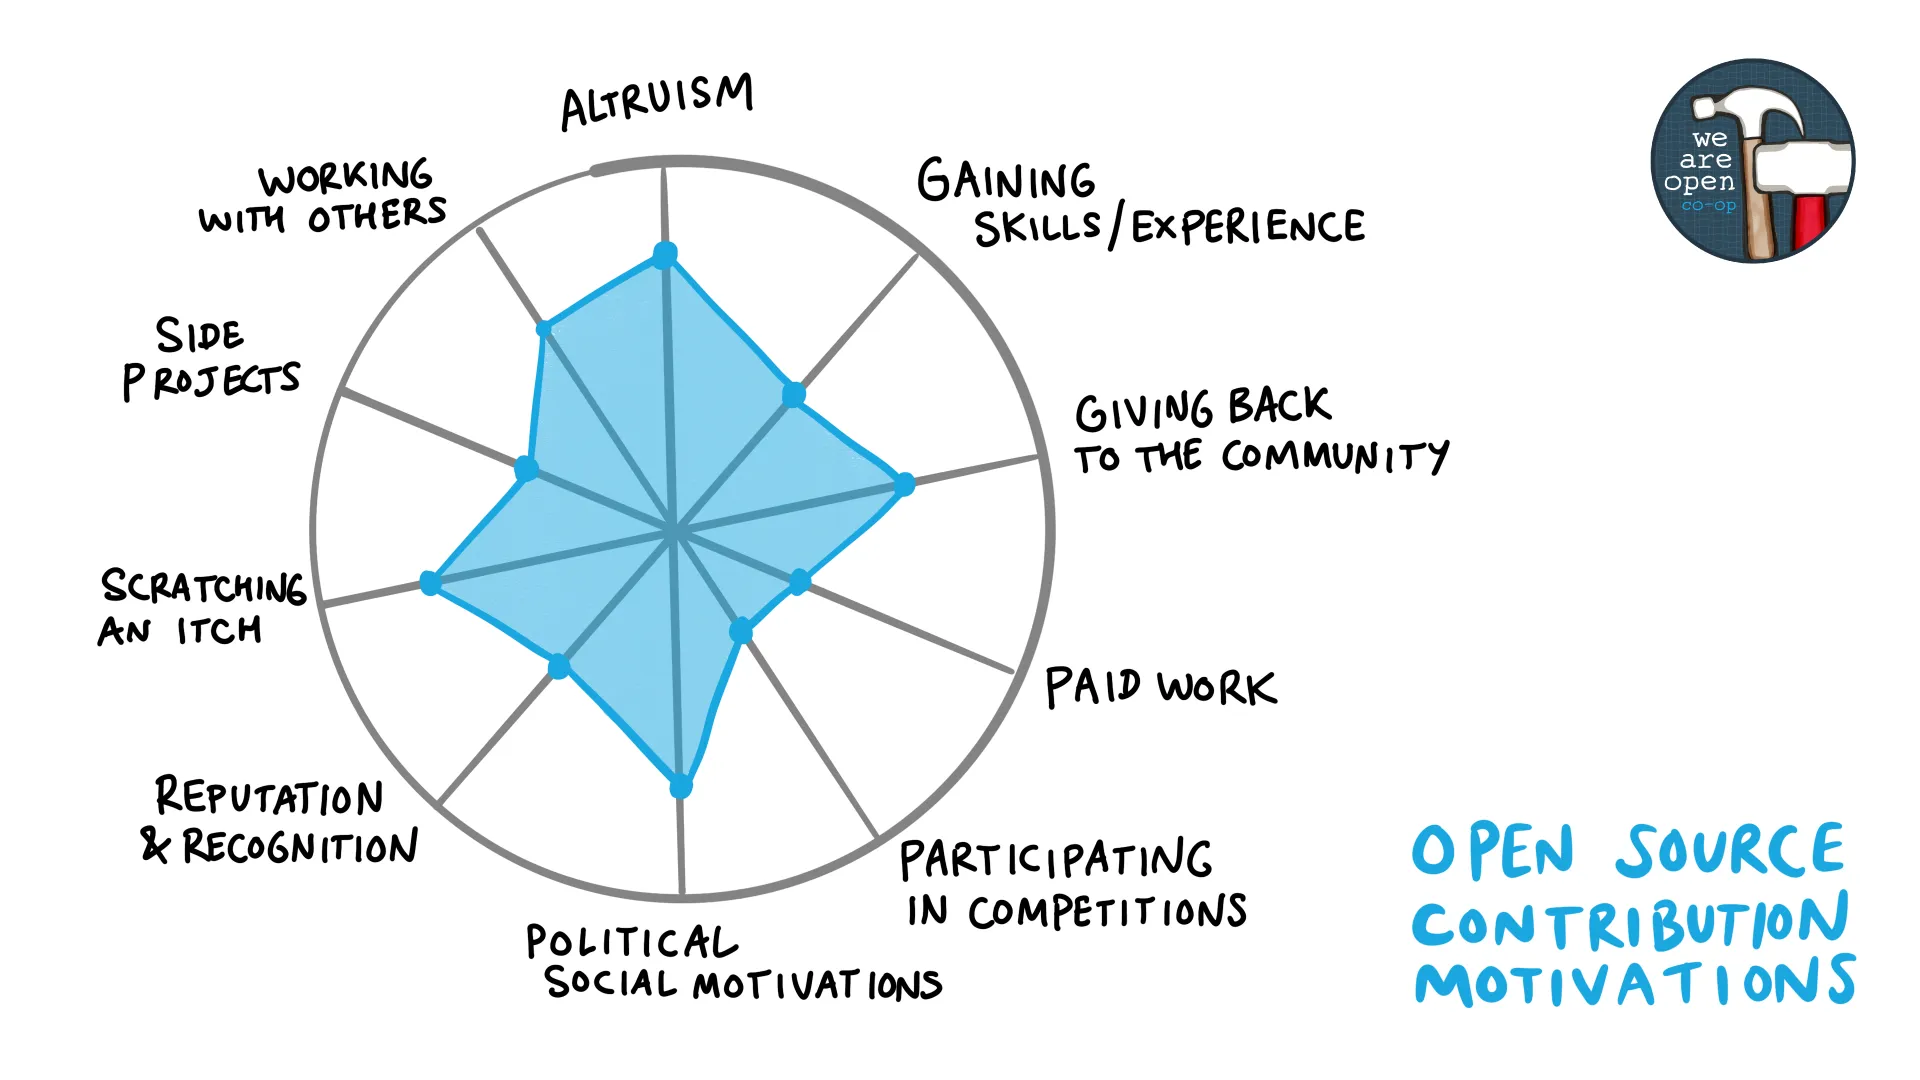
\includegraphics[width=0.9\textwidth]{figs/illustration.png}
    \caption{A quick look on motivations for contributing to open-source projects \cite{Belshaw_2020}}
    \label{fig:illustration}
\end{figure}

It is important to look at this subject for a number of reasons. Gaining an understanding of the motives of developers can help us guarantee the long-term viability of open-source initiatives. Furthermore, companies and organizations hoping to attract top talent within the open-source space would benefit from knowing what drives developer participation within these communities.  Uncovering these motivations can also shed light on how open-source projects function, how collaboration occurs, and how knowledge is shared and developed.

\subsection{Objectives}

This research project ventures beyond the surface of open-source software development, delving into the intricate web of motivations that drives developers within this collaborative community. By employing a multifaceted approach that combines empirical analysis with in-depth qualitative inquiries, the study seeks to illuminate the underlying forces that propel developers to contribute. These forces encompass not only the tangible incentives but also the value systems and socio-technical factors that influence their engagement. Ultimately, this investigation aims to provide a more nuanced understanding of the dynamics that shape the ever-evolving landscape of modern software development, with a specific focus on the crucial role played by open-source communities.

\subsection{Motivation}

As a former software engineer engrossed in the dynamic world of software development, my daily experience was enriched by the constant use of open-source software. From leveraging fundamental frameworks like ReactJS from Facebook to seamlessly integrating libraries and packages sourced from NPM, open-source solutions became an indispensable aspect of my workflow. Their ubiquitous presence became so ingrained in my routine that their influence often went unnoticed, seamlessly woven into the fabric of my daily tasks. However, as I transition into the realm of program software product management, I find myself drawn to exploring a new frontier – one that encompasses not only the technical aspects but also delves into the world of human psychology. It is this intersection of technology and human behavior that piques my curiosity and drives my desire to embark on this research endeavor.

Through this thesis, I aspire to investigate the nuanced interplay between open-source software adoption and the human factors influencing developer behavior and decision-making processes. By unraveling these complexities, I aim to contribute to a deeper understanding of how human elements shape the adoption, utilization, and evolution of open-source software, ultimately informing more effective software product management strategies.


\clearpage  % This command will start the next section from the new page
